\documentclass[12pt]{article}

% Packages for formatting
\usepackage[margin=1in]{geometry} % Set margins
\usepackage{amsmath} % For mathematical symbols
\usepackage{graphicx} % For including images
\usepackage{listings} % For including code
\usepackage{color} % For coloring code
\usepackage{hyperref} % For hyperlinks

% Define colors for code listing
\definecolor{codegreen}{rgb}{0,0.6,0}
\definecolor{codegray}{rgb}{0.5,0.5,0.5}
\definecolor{codepurple}{rgb}{0.58,0,0.82}
\definecolor{backcolour}{rgb}{0.95,0.95,0.92}

% Code listing styling
\lstdefinestyle{mystyle}{
    backgroundcolor=\color{backcolour},   
    commentstyle=\color{codegreen},
    keywordstyle=\color{magenta},
    numberstyle=\tiny\color{codegray},
    stringstyle=\color{codepurple},
    basicstyle=\ttfamily\footnotesize,
    breakatwhitespace=false,         
    breaklines=true,                 
    captionpos=b,                    
    keepspaces=true,                 
    numbers=left,                    
    numbersep=5pt,                  
    showspaces=false,                
    showstringspaces=false,
    showtabs=false,                  
    tabsize=2
}

\lstset{style=mystyle}

\title{ELCT 562 PA8}
\author{JACOB VAUGHT}
\date{\today}

\begin{document}

\maketitle


\section*{OFDM System Parameters}
\begin{figure}[ht]
\centering
\begin{minipage}{.5\textwidth}
  \centering
  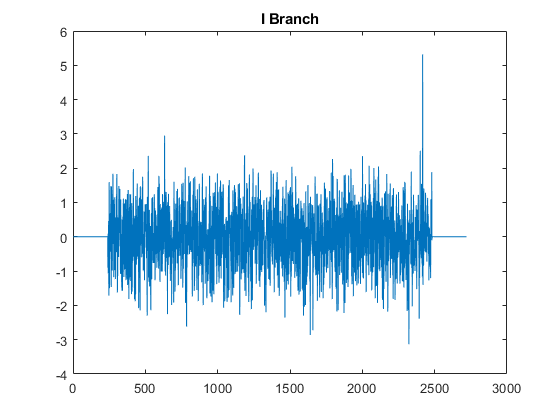
\includegraphics[width=.9\linewidth]{IB.png}
  \caption{In Phase Branch}
  \label{fig:first_image}
\end{minipage}%
\begin{minipage}{.5\textwidth}
  \centering
  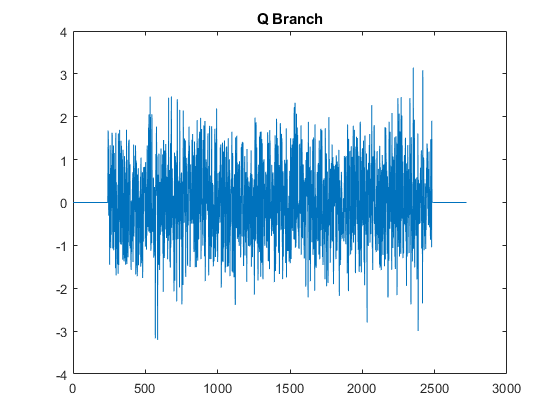
\includegraphics[width=.9\linewidth]{QB.png}
  \caption{Quadrature Branch}
  \label{fig:second_image}
\end{minipage}
\end{figure}
\begin{figure}[ht]
\centering

\includegraphics[width=0.8\textwidth]{PSD.png}
\caption{Power Spectral Density}
\label{fig:image1}
\end{figure}

\begin{enumerate}
    \item There would be 26 total number of OFDM symbols in the packet (\(S\)).
    
    \item Total number of samples per OFDM symbol including the cyclic prefix is given by:
    \[ N_{\text{total}} = (N + N_{cp}) \times S = 2080 \]
    
    \item The size of the FFT (IDFT/DFT) used in the system is:
    \[ IDFT/DFT = N = 64 \]
    
    \item The amount of samples in the cyclic prefix (CP) is 16. If the CP duration was shorter than the maximum excess delay of the multipath, then the OFDM signal would be degraded and the orthogonality of the subcarriers would be lost.
    
    \item Secret Message: "The fundamental problem of communication is that of reproducing at one point either exactly or approximately a message selected at another point." (C. Shannon, 1948)
\end{enumerate}

\section{Algorithm to Detect the Beginning of the Received Packet}
In the provided code, the beginning of the received packet is detected using a correlation-based method, specifically designed for timing synchronization in OFDM systems:

\begin{lstlisting}[language=Matlab]
for n = 1:numel(P)
    for m = 0:L-1
        P(n) = P(n) + r(n+m)*conj(r(n+m+L));
        R(n) = R(n) + r(n+m+L)*conj(r(n+m+L));
    end
end

Mn = abs(P).^2./abs(R).^2;
ind = find(Mn > 0.99); 
Nchoosen = ind(end);
\end{lstlisting}

Here, the algorithm calculates two sequences, \( P \) and \( R \), over a sliding window across the received signal \( r \). For each position \( n \), \( P \) is the sum of products of each pair of samples spaced \( L \) samples apart (half the FFT size, suggesting a relation to the cyclic prefix), and \( R \) is the energy of the signal segment following each position by \( L \) samples. The metric \( Mn \), the ratio of the squared magnitude of \( P \) to the squared magnitude of \( R \), peaks when the autocorrelation is strong, indicating the start of a repeated pattern such as the cyclic prefix in OFDM. The last index \( n \) where \( Mn \) exceeds a threshold (in this case, 0.99) is chosen as the start of the OFDM packet.

\begin{figure}[ht]
\centering
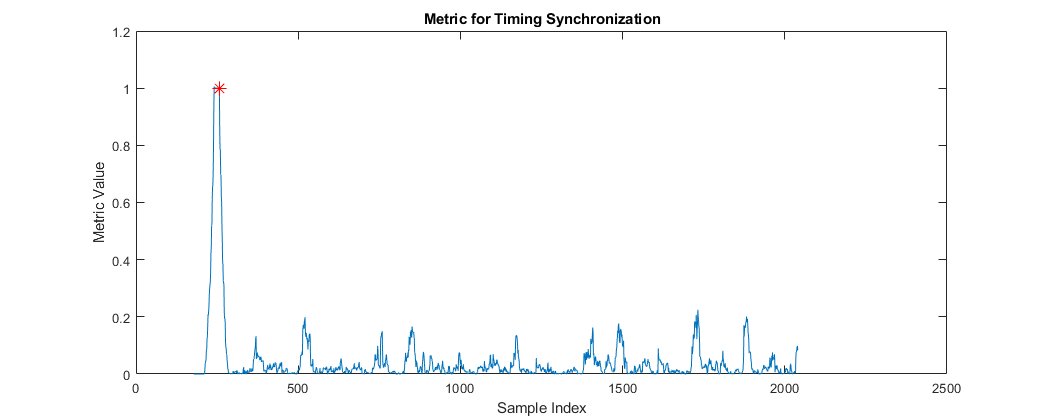
\includegraphics[width=0.9\textwidth]{metric.png}
\caption{Timing Synchronization}
\label{fig:image1}
\end{figure}


\section{Algorithm that Estimates the Carrier Frequency Offset (CFO)}
The carrier frequency offset is estimated using the phase of the correlation peak identified in the timing synchronization step:

\begin{lstlisting}[language=Matlab]
thetaCFO = P(Nchoosen) / abs(P(Nchoosen));
fcfoEst = -angle(thetaCFO) / (2 * pi * L) * Fsample;
\end{lstlisting}

Here, \( \theta_{\text{CFO}} \) is calculated as the phase of the correlation value \( P \) at the chosen starting index \( N_{\text{choosen}} \). This phase contains the frequency offset due to the relation between the transmitted and received symbols influenced by CFO. The estimated frequency offset \( f_{\text{cfoEst}} \) is then calculated by taking the angle of \( \theta_{\text{CFO}} \), scaling by the sample duration, and adjusting by the factor of \( 2\pi L \) to convert from phase to frequency.


\section{Frequency Offset Correction Method}
The frequency offset correction is performed by multiplying the received signal by a complex exponential that negates the estimated carrier frequency offset:

\begin{lstlisting}[language=Matlab]
rCorrected = r .* exp(-1i * 2 * pi * fcfoEst * [0:length(r)-1]' * Tsample);
\end{lstlisting}

In this line, \( r_{\text{Corrected}} \) is the frequency-corrected signal. The complex exponential \( \exp(-1i \cdot 2 \pi \cdot f_{\text{cfoEst}} \cdot [0:\text{length}(r)-1]' \cdot T_{\text{sample}}) \) represents a continuous-time complex sinusoid that rotates in the opposite direction of the estimated frequency offset. Multiplying the original signal by this term compensates for the frequency shift caused by the CFO.


\section{Multipath Channel Estimation}
The channel is estimated using the first OFDM symbol, assumed to contain known pilot data:

\begin{lstlisting}[language=Matlab]
HCFRe = symbolsWithoutEqualization(:, 1);
HCFRe(mod(k, N) + 1, :) = HCFRe(mod(k, N) + 1, :) ./ [Ga Gb].';
\end{lstlisting}

In this portion of the code, \( \text{symbolsWithoutEqualization} \) are the received OFDM symbols transformed into the frequency domain. The first column, corresponding to the first symbol, is used for channel estimation. This estimation uses known pilot values (encoded with Golay sequences \( G_a \) and \( G_b \)) to derive the channel frequency response by dividing the received pilot symbols by the transmitted pilot symbols. The result, \( H_{\text{CFRe}} \), represents the estimated channel frequency response.

\begin{figure}[ht]
\centering
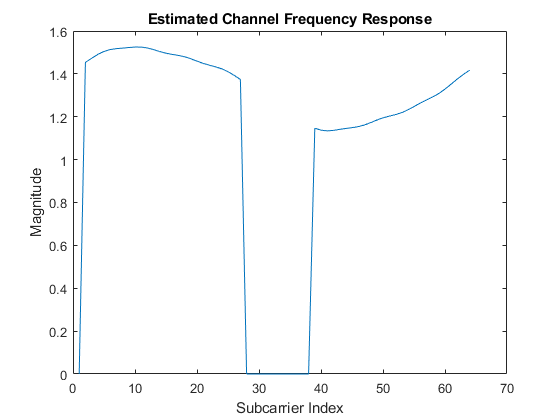
\includegraphics[width=0.5\textwidth]{chf.png}
\caption{Channel Frequency Response}
\label{fig:image1}
\end{figure}


\section{Equalization Method}
The equalization is performed to compensate for the channel effects:

\begin{lstlisting}[language=Matlab]
symbolsAfterEqualization = symbolsWithoutEqualization ./ HCFRe;
\end{lstlisting}

Here, \( \text{symbolsAfterEqualization} \) are obtained by dividing the frequency-domain received symbols by the estimated channel response, \( H_{\text{CFRe}} \). This operation corrects for channel-induced distortions, effectively flattening the frequency response seen by the transmitted data symbols.

\section{Detection Method to Obtain the Message Bits}
The received bits are determined from the equalized symbols based on the constellation mapping rules for BPSK:

\begin{lstlisting}[language=Matlab]
bitsRX = (real(symbolsAfterEqualization) > 0);
\end{lstlisting}

In BPSK (Binary Phase Shift Keying), the real part of the symbol determines the bit value. Symbols with a positive real part are interpreted as binary 1, while symbols with a negative real part are interpreted as binary 0. This straightforward detection method is aligned with the principles of BPSK modulation where the phase of the carrier wave is shifted to represent data bits.
\begin{figure}[ht]
\centering
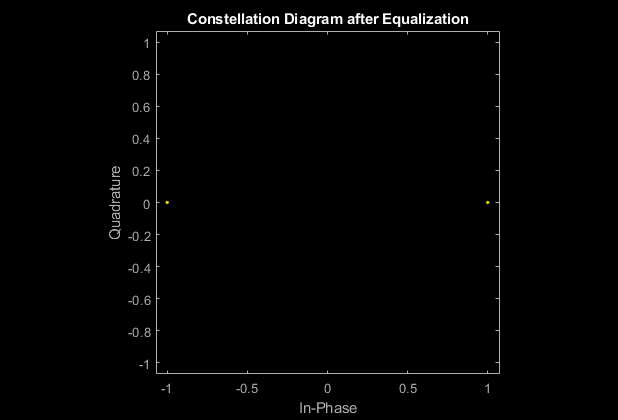
\includegraphics[width=0.8\textwidth]{const.png}
\caption{Constellation for BPSK}
\label{fig:image1}
\end{figure}

\newpage
\section{MATLAB Code}
\begin{lstlisting}[language=Matlab]
% Clear workspace and close all figures
clear;
close all;

% Load IQ data from a MATLAB file
load('RXIQdata.mat');

% Define OFDM parameters
S = 26;                     % Total number of OFDM symbols 
M = 52;                     % Number of subcarriers
Fspacing = 312.5E3;         % Subcarrier spacing
Fsample = 20E6;             % Sampling frequency
Tsample = 1/Fsample;        % Sampling period
N = Fsample/Fspacing;       % FFT size
CP_len = N/4;               % Cyclic prefix length
Ga = [1 1 1 1 -1 1 1 -1 -1 1 -1 1 -1 1 -1 -1 1 -1 1 1 1 -1 -1 1 1 1]; % Golay sequence A
Gb = [1 1 1 1 -1 1 1 -1 -1 1 -1 1 1 1 1 1 -1 1 -1 -1 -1 1 1 -1 -1 -1]; % Golay sequence B
k = [-26:-1 1:26];          % Subcarrier indices
kSynch = [-26:2:-1 0:2:25]; % Synchronization subcarrier indices
Toffset = 20e-6;            % Timing offset
Tend = 20e-6;               % End time
Noffset = floor(Toffset/Tsample); % Number of samples offset
Nroom = 5;                  % Room for timing offset
Nend = floor(Tend/Tsample); % End sample index
hCIR = zeros(N,1);          % Channel impulse response initialization
fcfo = 43e3;                % Carrier frequency offset for simulation

% Symbol and cyclic prefix durations
Tsym = 1/Fspacing;
Tcp = Tsym/4;
Ncp = Tcp/Tsample;

% Generation of synchronization symbols
synchSymbols = 2 * randi([0 1], M/2, 1) - 1;

% Flatten the received signal array for processing
r = RXIQdata(:);

% Coarse timing synchronization
L = N/2;                    % Half the FFT size for timing metric
P = zeros(2040, 1);         % Correlation between received signal segments
R = zeros(2040, 1);         % Energy of delayed received signal segments

for n = 1:numel(P)
    for m = 0:L-1
        P(n) = P(n) + r(n+m) * conj(r(n+m+L));
        R(n) = R(n) + r(n+m+L) * conj(r(n+m+L));
    end
end

Mn = abs(P).^2 ./ abs(R).^2;  % Metric for timing detection
ind = find(Mn > 0.99);        % Indices where metric exceeds threshold

Nchoosen = ind(end);          % Choose the last index where condition is met

% CFO estimation
thetaCFO = P(Nchoosen) / abs(P(Nchoosen));  % Phase of the correlation at chosen index
fcfoEst = -angle(thetaCFO) / (2 * pi * L) * Fsample;  % Estimated CFO
rCorrected = r .* exp(-1i * 2 * pi * fcfoEst * [0:length(r)-1]' * Tsample);  % Corrected received signal

% Channel estimation using the first OFDM symbol
Nsync = Nchoosen - Nroom + N;
dataSymbols = 2 * randi([0, 1], M, S) - 1;  % Generate data symbols for simulation

% Equalization process
Npacket = (N + Ncp) * (S + 1);  % Total number of samples per packet
rOFDMwithCP = reshape(rCorrected(Nsync + [0:Npacket-1]), N + Ncp, []);  % Separate packets including CP
rOFDMwithoutCP = rOFDMwithCP(Ncp + 1:end, :);  % Remove cyclic prefix
X = 1/sqrt(N) * dftmtx(N)';  % Normalized DFT matrix
symbolsWithoutEqualization = X' * rOFDMwithoutCP;  % Transform to frequency domain
HCFRe = symbolsWithoutEqualization(:, 1);  % Channel response estimate from first symbol
HCFRe(mod(k, N) + 1, :) = HCFRe(mod(k, N) + 1, :) ./ [Ga Gb].';  % Apply Golay sequences for channel estimation

% Equalize the symbols using the estimated channel response. This involves dividing the frequency domain received symbols by the estimated channel response to mitigate the effects of the channel.
symbolsAfterEqualization = symbolsWithoutEqualization ./ HCFRe;
symbolsAfterEqualization = symbolsAfterEqualization(mod(k, N) + 1, 2:end); % Remove first column (used for channel estimation) and correct index

% BPSK Demodulation
% Convert the equalized symbols into bits by checking if they are greater than zero
bitsRX = (real(symbolsAfterEqualization) > 0);

% Convert the received bits into a string
% First, convert the logical array to characters ('0' or '1'), then reshape and convert binary to decimal, finally convert to characters
str = char(bin2dec(reshape(char(bitsRX(:) + '0'), 8, []).')).';
\end{lstlisting}


\end{document}